\mode*


\begin{frame}
\frametitle{What is Double Machine Learning (DML)?}
%\begin{itemize}
%\item \textbf{DML} combines econometrics and machine learning
%\item \textbf{Exploiting the strengths of two disciplines}:
%\end{itemize}
%\vspace*{-10pt}
\begin{center}
\pdftooltip{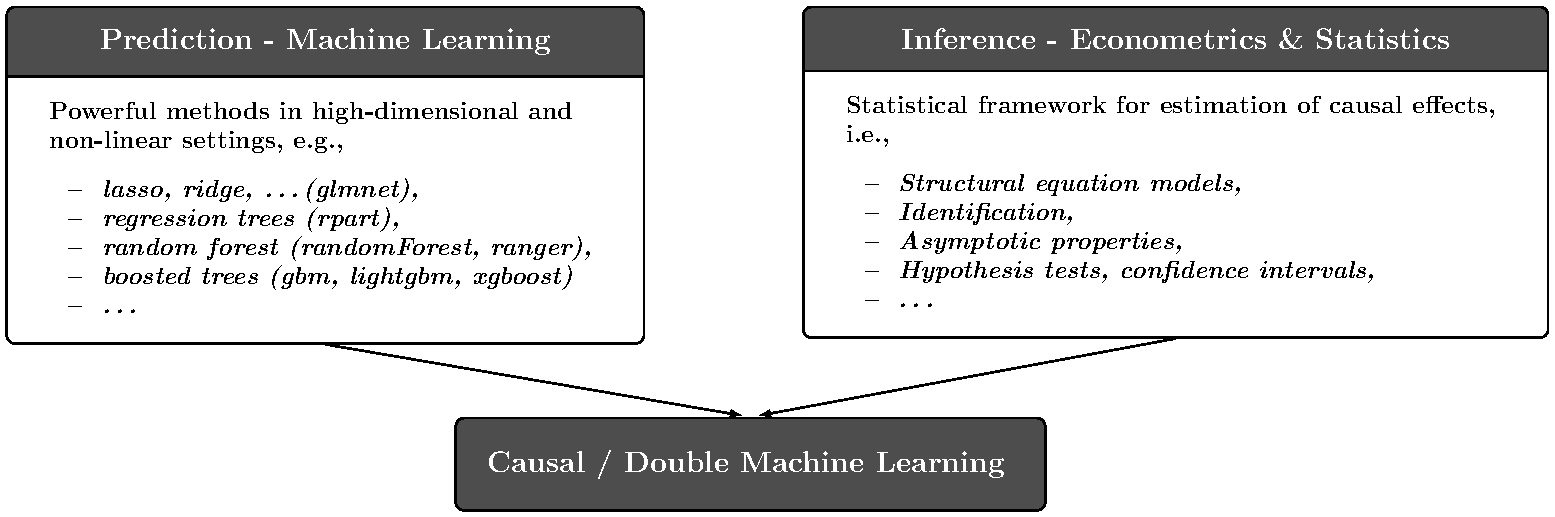
\includegraphics[width = \textwidth]{workflow/doubleml_ml_eco_useR.pdf}}{
A diagram with three boxes. On top, there are two boxes. On the left, a box with title PREDICTION - MACHINE LEARNING; on the right a box with title INFERENCE - ECONOMETRICS AND STATISTICS. In the first box (prediction) it is written: Powerful methods in high-dimensional and non-linear settings, for example, lasso, ridge, regression trees, random forests and boosted trees. In the second box (inference) it is written: Statistical framework for estimation of causal effects, this is, structural equation models, identification, asymptotic theory, hypothesis tests and confidence intervals.}
\end{center}
%\begin{itemize}
%\item \textbf{Machine Learning}: Prediction in high-dimensional non-linear settings
%\item \textbf{Econometrics}: Causality, identification, asymptotic properties of estimators
%\end{itemize}
\begin{itemize}
\item \textbf{Result / output} from the DML framework:
\begin{itemize}
\item Estimate of a causal effect or structural parameter with valid confidence intervals $\rightarrow$ statistical tests for parameter(s) of interest
\item Good statistical properties ($\sqrt{N}$ rate of convergence; unbiased; approximately Gaussian)
%\item Multiple treatment effects; heterogeneous treatment effects, \ldots
\end{itemize}
\end{itemize}
\end{frame}


\begin{frame}
\frametitle{Causal Machine Learning: Examples}
\begin{itemize}
\item Evaluation of an intervention in randomized controlled trials or observational studies, e.g., A/B testing, clinical studies, program evaluation
\item General: What is the \textbf{effect} of a certain \textbf{treatment} on a relevant \textbf{outcome} variable?
%\item A \textbf{randomized experiment} is a direct way to estimate a \textbf{causal effect} (assuming it is conducted properly)
\vspace{10pt}
\end{itemize}
\begin{center}
\pdftooltip{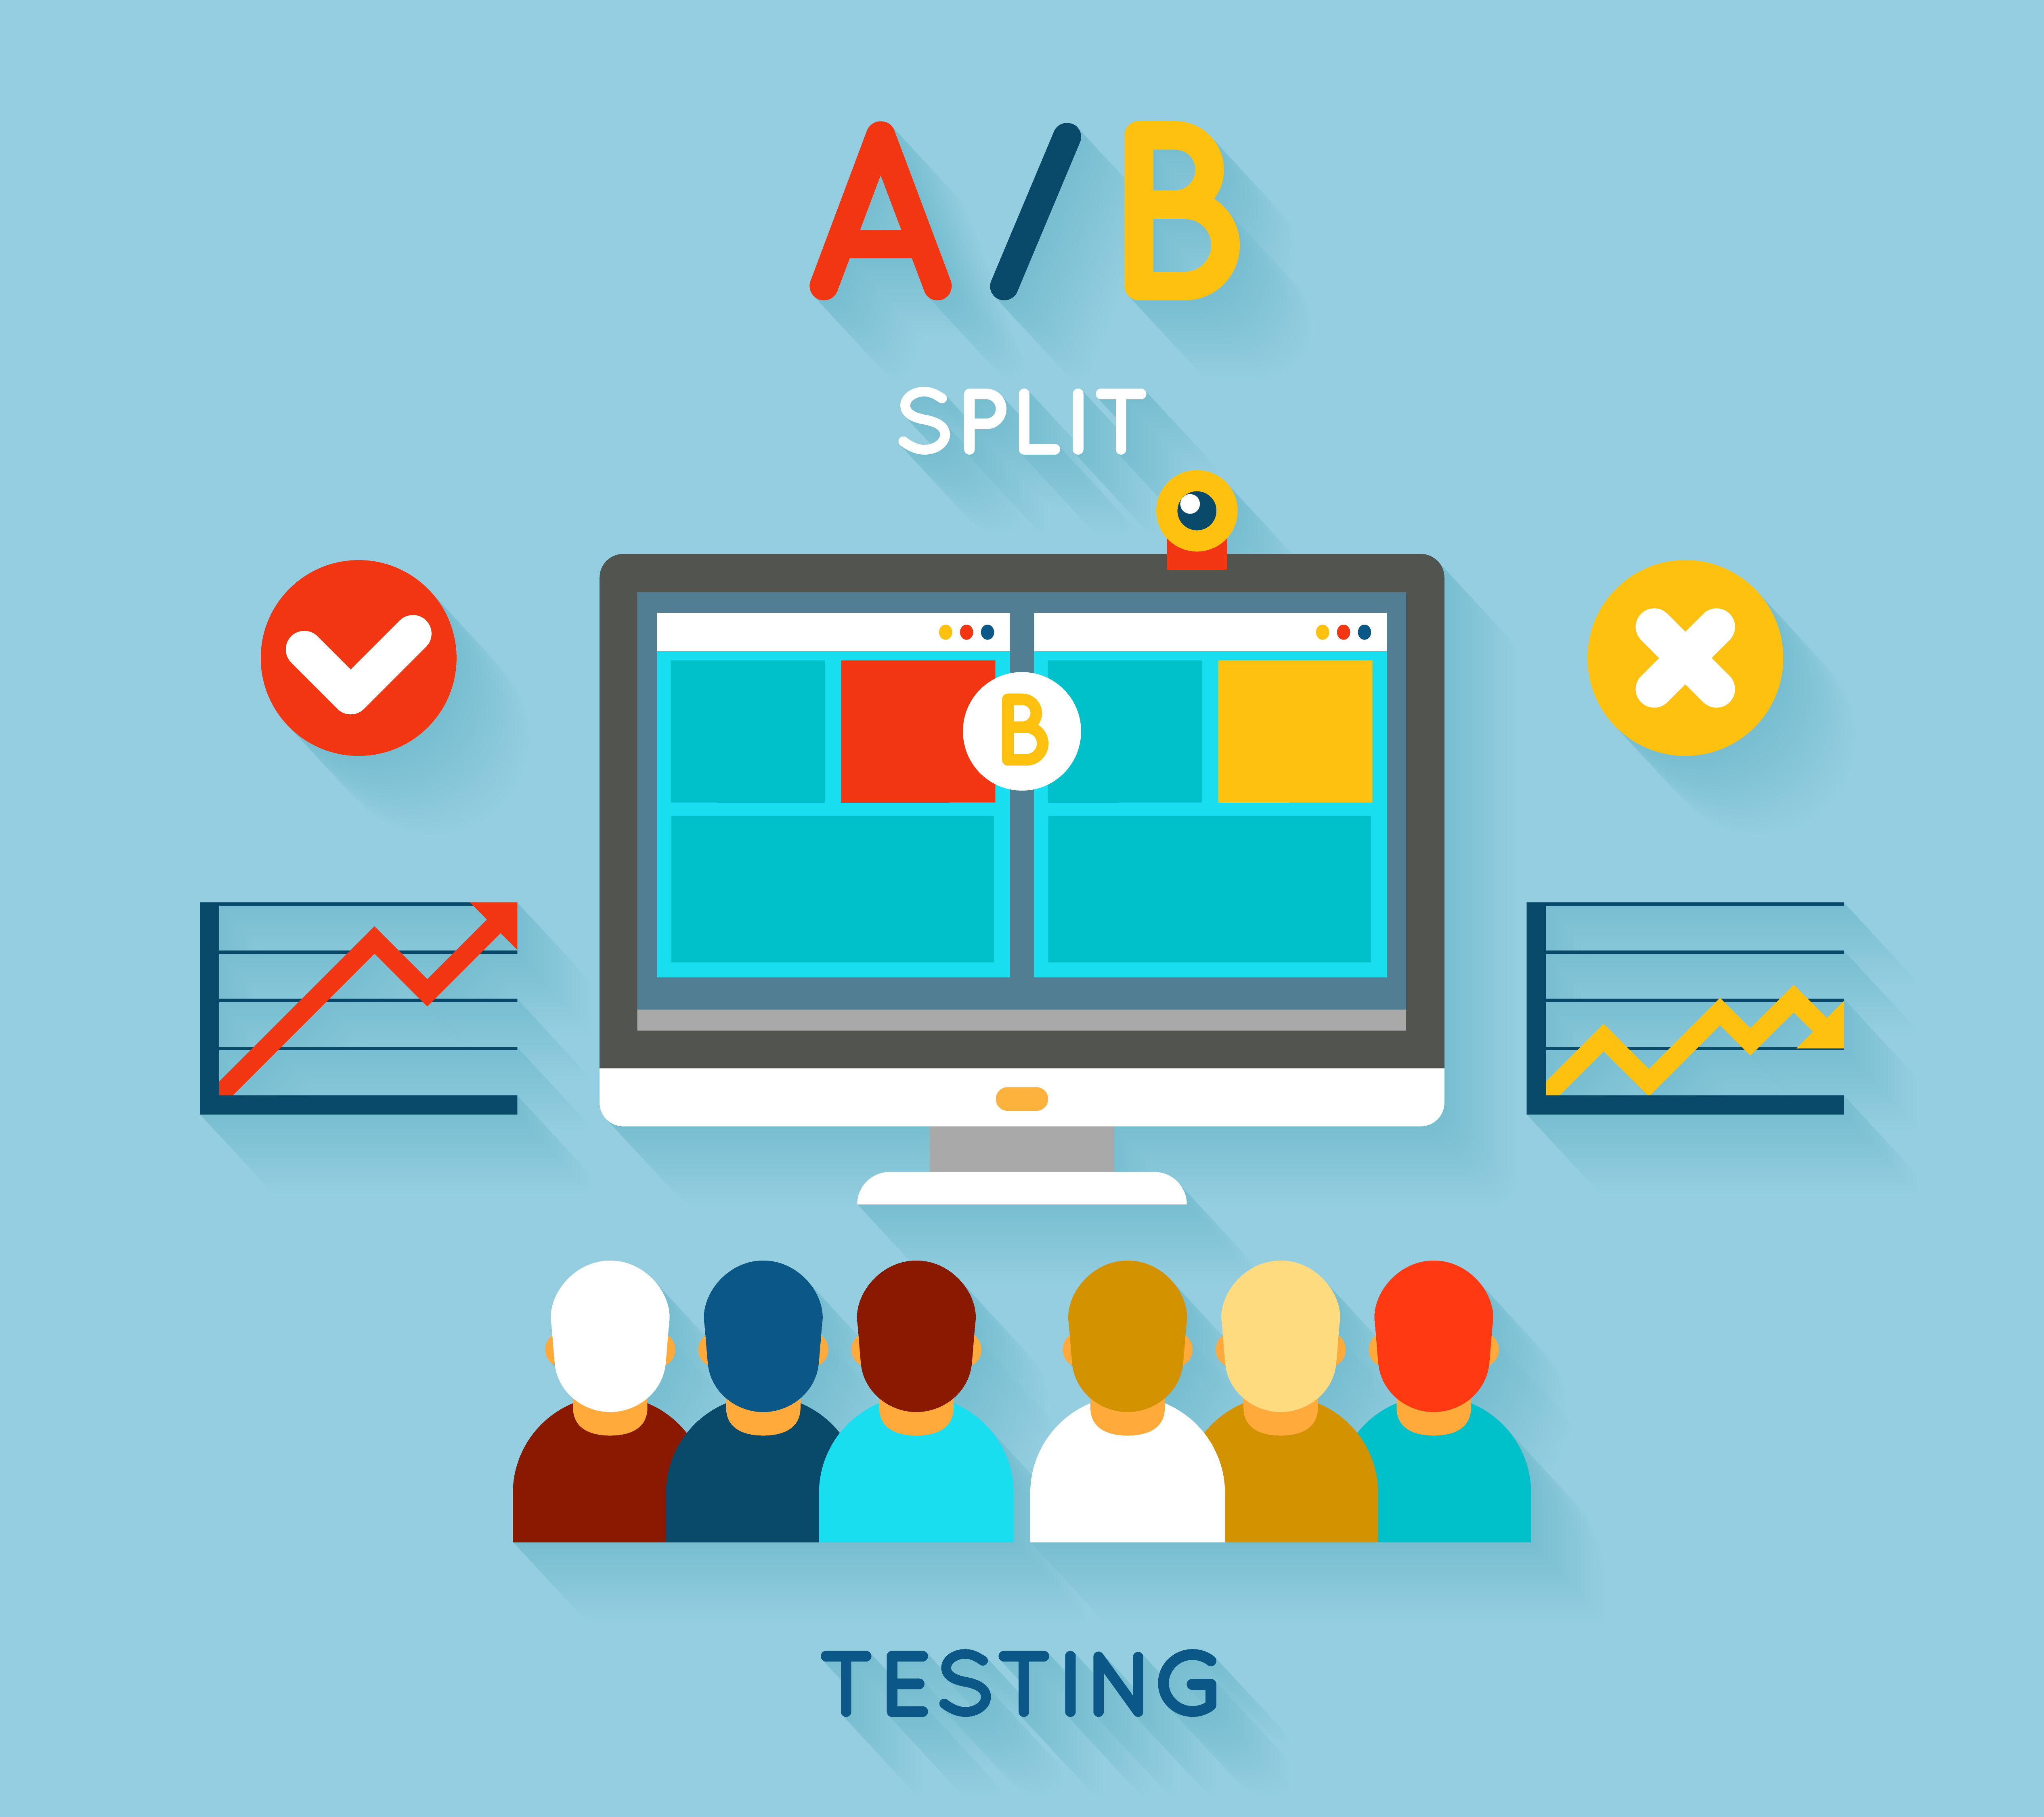
\includegraphics[width=0.4\textwidth]{pictures_and_logos/ab_testing.jpg}}{An illustration of A/B testing. Stylized persons look on a split screen. On the left hand side of the screen there is a window with an orange rectangle (illustrating version A). On the right hand side of the screen there is a window with a yellow rectangle (illustrating version B). To the left of the screen there is a graph with an increasing red curve and a check mark above. On the right of the screen, there is stagnating yellow graph and a cross above.}
\end{center}
{\tiny \hfill Image Source: Freepik (\url{http://www.freepik.com}) / Designed by macrovector}
\end{frame}

%\begin{frame}
%\frametitle{Example: Partially Linear Regression}
%\begin{itemize}
%\item Partially linear regression (PLR) model
%\begin{align*}
%Y = D\theta_0 + g_0(X) + \zeta, \quad \mathbb{E}(\zeta|D,X)=0,
%\end{align*}
%with potentially non-linear function $g_0(X)$ and 
%\begin{itemize}
%\item $Y$ - outcome variable,
%\item $D$ - treatment variable, 
%\item $X = (X_1,\ldots, X_p)$ - potentially high-dimensional vector of confounding variables.
%\end{itemize}
%\end{itemize}
%\vspace{10pt}
%\begin{center}
%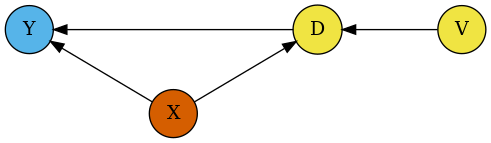
\includegraphics[width=0.6\textwidth]{pictures_and_logos/dag_plr2.png}
%\end{center}
%\end{frame}
%
